% Copyright (c)  2005-2010 EDF-EADS-PHIMECA.
% Permission is granted to copy, distribute and/or modify this document
% under the terms of the GNU Free Documentation License, Version 1.2
% or any later version published by the Free Software Foundation;
% with no Invariant Sections, no Front-Cover Texts, and no Back-Cover
% Texts.  A copy of the license is included in the section entitled "GNU
% Free Documentation License".
\renewcommand{\filename}{docUC_InputNoData_UsualDist}
\renewcommand{\filetitle}{UC : List of usual distributions}

% \HeaderNNIILevel
% \HeaderIILevel
\HeaderIIILevel

\index{Usual Distribution!Arcsine}
\index{Usual Distribution!Beta}
\index{Usual Distribution!Bernoulli}
\index{Usual Distribution!Binomial}
\index{Usual Distribution!Burr}
\index{Usual Distribution!Chi}
\index{Usual Distribution!ChiSquare}
\index{Usual Distribution!Dirichlet}
\index{Usual Distribution!Epanechnikov}
\index{Usual Distribution!Exponential}
\index{Usual Distribution!Fisher-Snedecor}
\index{Usual Distribution!Gamma}
\index{Usual Distribution!Gumbel}
\index{Usual Distribution!Histogram}
\index{Usual Distribution!InverseNormal}
\index{Usual Distribution!Laplace}
\index{Usual Distribution!Logistic}
\index{Usual Distribution!LogNormal}
\index{Usual Distribution!LogUniform}
\index{Usual Distribution!Negative Binomial}
\index{Usual Distribution!Non Central Chi Square}
\index{Usual Distribution!Non Central Student}
\index{Usual Distribution!Normal}
\index{Usual Distribution!Rayleigh}
\index{Usual Distribution!Rice}
\index{Usual Distribution!Student}
\index{Usual Distribution!Triangular}
\index{Usual Distribution!Trapezoidal}
\index{Usual Distribution!TruncatedNormal}
\index{Usual Distribution!Uniform}
\index{Usual Distribution!Weibull}
\index{Usual Distribution!Geometric}
\index{Usual Distribution!Multinomial}
\index{Usual Distribution!Poisson}
\index{Usual Distribution!User defined}
\index{Distribution!Usual distribution}
\index{Distribution!Zipf-Mandelbrot}



The objective of this Use Case is to list all the usual distributions proposed by Open TURNS and to precise how each distribution is created, with its different arguments.\\

The different distributions proposed by Open TURNS are listed here after.\\[1em]

Details on each object may be found in the User Manual  (\href{OpenTURNS_UserManual_TUI.pdf}{see User Manual - Probabilistic modeling / Usual Distributions}).\\[1em]

\begin{itemize}
\item Continuous distributions :
\end{itemize}

{\footnotesize
  \noindent \begin{tabular}{|p{1.8cm}|p{6.0cm}|p{2.7cm}|p{1.7cm}|p{4.6cm}|}
    % 
    \hline
    % 
    Name & probability density function & conditions & param. 1 & param. $2^{\strut}_{\strut}$\\
    % 
    \hline
    % 
    Arcsine & $\frac{1}{\pi \frac{b-a}{2} \sqrt{1-\left(\frac{x-\frac{a+b}{2}}{\frac{b-a}{2}}\right)^{2}}}$ & $a <b$& $(a, b)$ & $(\mu, \sigma)$ with
    $
    \left\{
      \begin{array}{l}
        \mu = \frac{a+b}{2} \\
        \sigma = \frac{b-a}{2\sqrt{2}}
      \end{array}
    \right.
    $ \\
    % 
    \hline
    % 
    Beta & $\displaystyle  \frac{(x-a)^{(r-1)^{\strut}}(b-x)^{(t-r-1)}}{(b-a)^{(t-1)}B(r,t-r)}\boldsymbol{1}_{[a,b]}(x)$  & $r>0$, $t>r$, $a < b$ & $(r, t, a, b)$ & $(\mu, \sigma, a,b)$ with

    $
    \left\{
      \begin{array}{l}
        \mu = a+(b-a)\frac{r}{t} \\
        \sigma = (b-a)\frac{r}{t}\frac{\sqrt{t-r}}{\sqrt{r(t+1)}}
      \end{array}
    \right._{\strut}
    $\\
    % 
    \hline
    % 
    Burr & $\displaystyle ck\frac{x^{(c-1)}}{(1+x^c)^{(k+1)}} \boldsymbol{1}_{]0,+\infty[}(x)$  & $c>0$, $k>0$,  & $(c,k)$ & - \\
    % 
    \hline
    % 
    Chi & $\displaystyle x^{\nu-1}e^{-x^2/2}\frac{2^{1-\nu^{\strut}/2}}{\Gamma(\nu/2)_{\strut}} \boldsymbol{1}_{[0,+\infty[}(x)$ & $\nu > 0$& $\nu$ & -- \\
    % 
    \hline
    % 
    ChiSquare & $\displaystyle \frac{2^{-\nu^{\strut}/2}}{\Gamma(\nu/2)_{\strut}} x^{(\nu/2-1)}e^{-x/2}\boldsymbol{1}_{[0,+\infty[}(x)$ & $\nu > 0$& $\nu$ & -- \\
    % 
    \hline
    % 
    Dirichlet & $\displaystyle A \left[ 1-\sum_{j=1}^{d} x_j\right]^{(\theta_{d+1}-1)}\prod_{j=1}^d x_j^{(\theta_j-1)}\mathbf{1}_{\Delta}(\vect{x}) $ with $A = \frac{\Gamma(\sum_{j=1}^{d+1}\theta_j)}{\prod_{j=1}^{d+1}\Gamma(\theta_j)}$, $\Delta = \{ \vect{x} \in \mathbb{R}^d / \forall i, x_i \geq 0, \sum_{i=1}^{d} x_i \leq 1 \}$ & $d \geq 1$, $\theta_i>0$ & $(\theta_1, \hdots, \theta_{d+1})$  & -- \\
    % 
    \hline
    % 
    Epanechnikov & $\displaystyle \frac{3^{\strut}}{4_{\strut}}(1 - x^2)\boldsymbol{1}_{[-1,1]}(x)$ & -- & -- & -- \\
    % 
    \hline
    % 
    Exponential & $ \displaystyle \lambda e^{-\lambda(x-\gamma)^{\strut}}\boldsymbol{1}_{[\gamma,+\infty[_{\strut}}(x)$ & $\lambda>0$ & $(\lambda, \gamma)$ & - \\
    % 
    \hline
    % 
    Fisher-Snedecor & \tiny$\displaystyle  \left[\left(\frac{d_1x}{d_1x+d_2}\right)^{d_1/2} \left(\frac{d_2}{d_1x+d_2}\right)^{{d_2/2}^{\strut}} \right]\frac{\mathbf{1}_{x \geq 0}}{Ax} $ with $A =  B(d_1/2, d_2/2)$ & $d_i>0$ & $\left(d_1, d_2 \right)_{\strut}$ & -- \\
    % 
    \hline
    % 
    Gamma & $ \displaystyle \frac{\lambda^{k^{\strut}}}{\Gamma(k)_{\strut}}(x-\gamma)^{(k-1)} e^{-\lambda(x-\gamma)}\boldsymbol{1}_{[\gamma,+\infty[}(x)$ & $k>0$, $\lambda > 0$ & $(k, \lambda, \gamma)$ & $(\mu, \sigma, \gamma)$ with
    $
    \left\{
      \begin{array}{l}
        \mu = \frac{k}{\lambda} +  \gamma \\
        \sigma = \frac{\sqrt{k}}{\lambda}
      \end{array}
    \right.
    $\\
    % 
    \hline
    % 
    Gumbel & $ \displaystyle \alpha e^{-\alpha(x-\beta)-e^{-\alpha(x-\beta)}}$ & $\alpha >0 $ & $(\alpha, \beta)$ & $(\mu, \sigma)$ with $
    \left\{
      \begin{array}{l}
        \mu = \frac{\gamma^{*}}{\alpha} + \beta \\
        \sigma = \frac{\pi}{\sqrt{6}} \frac{1}{\alpha}
      \end{array}
    \right.^{\strut}
    $
    where $ \displaystyle \gamma^{*} = -\int_0^{\infty} \log(t)e^{-t}dt$ is Euler's constant.
    \\
    % 
    \hline
    % 
    Histogram & $ \displaystyle \sum_{i=1}^{n} h_i1_{[x_i, x_{i+1}]}(x)/S $ & $\begin{array}{lcl}
      l_i^{\strut} & = & x_{i+1} - x_i\\
      S & = & \sum_{i=1}^n h_i l_i \\
      l_i & \geq & 0
    \end{array}
    $ & $(x_1, (h_i, l_i))$ ${1\leq i \leq n} $ & -- \\
    % 
    \hline
    % 
    Inverse-Normal & $\displaystyle \left(\frac{\lambda}{2\pi x^3} \right)^{1/2}e^{-\lambda(x-\mu)^2/(2\mu^2x)} \mathbf{1}_{x>0}$ & $\lambda>0$, $\mu>0$ & $(\lambda, \mu)$ & -- \\
    % 
    \hline
    % 
    Laplace & $ \displaystyle \frac{\lambda^{\strut}}{2_{\strut}}e^{-\lambda |x-\mu|}$ & $\lambda>0$ & $(\lambda, \mu)$ & -- \\
    % 
    \hline
    % 
    Logistic & $ \displaystyle \frac{e^{\left(\frac{x-\alpha}{\beta}\right)^{\strut}}} {\beta\left(1+ e^{\left(\frac{x-\alpha}{\beta}\right)}\right)^2_{\strut}}\boldsymbol{1}_{[\alpha,+\infty[}(x) $ & $\beta > 0$ & $(\alpha, \beta)$ & -- \\
    % 
    \hline
    % 
    \ifpdf % Manual splitting of the tabular in PDF mode
  \end{tabular}\\

  \noindent \begin{tabular}{|p{2cm}|p{5.3cm}|p{2.7cm}|p{1.7cm}|p{4.6cm}|}
    % 
    \hline
    % 
    Name & probability density function & conditions & param. 1 & param. $2^{\strut}_{\strut}$\\
    % 
    \hline
    % 
    LogNormal & $ \displaystyle \frac{e^{-\frac{1}{2}\left(\frac{log(x-\gamma)-\mu_\ell}{\sigma_\ell}\right)^{2^{\strut}}}}{\sqrt{2\pi}\sigma_\ell (x-\gamma)}\boldsymbol{1}_{[\gamma,+\infty[}(x) $ & $\sigma_\ell >0$ & $(\mu_\ell, \sigma_\ell, \gamma)$ & $(\mu, \sigma, \gamma)$ or $(\mu, \frac{\sigma}{\mu}, \gamma)$ (param. 3) with
    $
    \left\{
      \begin{array}{@{}l@{}}
        \mu =  e^{\frac{1}{2}\sigma_\ell^2 + \mu_\ell} + \gamma\\
        \sigma =  (e^{\frac{1}{2}\sigma_\ell^2 + \mu_\ell})\sqrt{e^{\sigma_\ell^2}-1}
      \end{array}
    \right.
    $\\
    % 
    \hline
    % 
    LogUniform & $ \displaystyle \frac{1}{x(b_\ell-a_\ell)}\boldsymbol{1}_{[a_\ell, b_\ell]}(\log(x)) $ & $b_\ell > a_\ell$ & $(a_\ell, b_\ell)$ & -- \\
    % 
    \hline
    % 
    \else
    \fi
    Non Central Chi Square & $ \displaystyle \sum_{j=0}^{\infty} e^{-\lambda}\frac{\lambda^j}{j!}p_{\chi^2(\nu+2j)}(x)$ where $p_{\chi^2(q)}$ is the PDF of a $\chi^2(q)$ random variate.& $\nu>0$, $\lambda \geq 0$ & $(\nu,\lambda )$ & -- \\
    % 
    \hline
    % 
    Non Central Student & See text for $p_{NCS}(x)^{\strut}$ & -- & $(\nu,\delta, \gamma )$ & -- \\
    % 
    \hline
    % 
    Normal (nD) & $\displaystyle
    \frac{1}
    {
      \displaystyle (2\pi)^{\frac{n}{2}}(\mathrm{det}\mat{\Sigma})^{\frac{1}{2}}
    }
    \displaystyle e^{-\frac{1}{2}\Tr{(\vect{x}-\vect{\mu})}\mat{\Sigma}^{-1^{\strut}}(\vect{x}-\vect{\mu})}$
    &
    $\mat{\Sigma} = \mat{\Lambda}_{\vect{\sigma}} \mat{R} \mat{\Lambda}_{\vect{\sigma}}$, $\mat{\Lambda}_{\vect{\sigma}} = \mathrm{diag}(\vect{\sigma})$, $\mat{R}$ SPD, $\sigma_i >0$ & $(\vect{\mu}, \vect{\sigma},\mat{R})$ or $(\vect{\mu}, \mat{\Sigma})$ & -- \\
    % 
    \hline
    % 
    Rayleigh & $\displaystyle \frac{(x - \gamma)^{\strut}}{\sigma^2_{\strut}}e^{-\frac{(x-\gamma)^2}{2\sigma^2}}\boldsymbol{1}_{[\gamma,+\infty[}(x)$ & $\sigma > 0$ & $(\sigma, \gamma)$ & -- \\
    % 
    \hline
    % 
    Rice & $\displaystyle 2\frac{x}{\sigma_{\strut}^{2^{\strut}}}p_{\chi^2(2,\frac{\nu^2}{\sigma^2})}(\frac{x^2}{\sigma^2})$ where $p_{\chi^2(\nu, \lambda)}$ is the PDF of a Non Central Chi Square random variate $(\nu, \lambda)$. & $\nu \geq 0, \sigma>0$ & $( \sigma, \nu)$ & -- \\
    % 
    \hline
    % 
    Student (nD) & See text for $p_T(x)^{\strut}$ & $\nu > 2$ & $(\nu,\vect{\mu}, \vect{\sigma}, \mat{R}_{\strut} )$ & $(\nu, \mu, \sigma)$ with $d=1$ \\
    % 
    \hline
    % 
    Triangular & $  \displaystyle \left\{
      \begin{array}{ll}
        \displaystyle 2\frac{x-a}{(m-a)(b-a)} & a \leq x \leq m \\
        \displaystyle 2\frac{b-x}{(b-m)(b-a)} & m \leq x \leq b \\
        0 & \mbox{otherwise.}
      \end{array}
    \right.^{\strut} $ & $a < m < b$ & $(a, m, b)$ & - \\
    % 
    \hline
    % 
    Truncated Normal & $  \displaystyle \frac{\frac{1^{\strut}}{\sigma_n}\phi(\frac{x-\mu_n}{\sigma_n})}
    {\Phi(\frac{b-\mu_n}{\sigma_n}) - \Phi(\frac{a-\mu_n}{\sigma_n})}\boldsymbol{1}_{[a, b]}(x)$
    & $\sigma_n >0$ & $(\mu_n, \sigma_n, a, b)$ & - \\
    % 
    \hline
    % 
    Uniform & $  \displaystyle \frac{1^{\strut}}{b-a}\boldsymbol{1}_{[a, b]}(x)$ & $a < b$ & $(a, b)$ & -- \\
    % 
    \hline
    % 
    Weibull &  $\displaystyle \frac{\beta^{\strut}}{\alpha}\left(\frac{x-\gamma}{\alpha}\right)^{\beta-1}e^{-\left(\frac{x-\gamma}{\alpha}\right)^\beta} \boldsymbol{1}_{[\gamma,+\infty[}(x)$ & $\alpha>0$, $\beta>0$ &  $(\alpha, \beta, \gamma)$ & $(\mu, \sigma, \gamma)$ with
    $
    \left\{
      \begin{array}{@{}l@{}}
        \mu =  \alpha\Gamma(1+\frac{1}{\beta}) + \gamma\\
        \sigma =  \alpha\sqrt{\Gamma(1+\frac{2}{\beta}) - \Gamma^2(1+\frac{1}{\beta})}
      \end{array}
    \right._{\strut}
    $ \\
    % 
    \hline
    % 
  \end{tabular}
}\\

\vspace*{0.2cm}
Let's note that a random variable $X$ is said to have a standard non-central student distribution $\mathcal{T}(\nu, \delta)$ if it can be written as:
\begin{equation}
  X = \frac{N}{\sqrt{C/\nu}}
\end{equation}
where $N$ has the normal distribution $\mathcal{N}(\delta, 1)$ and $C$ has the $\chi^2(\nu)$ distribution, $N$ and $C$ being independent.\\
The non-central Student distribution in OpenTURNS has an additional parameter $\gamma$ such that the random variable $X$ is said to have a non-central Student distribution $\mathcal{T}(\nu, \delta, \gamma)$ if $X-\gamma$ has a standard $\mathcal{T}(\nu,\delta)$ distribution.\\

We explicitate here the probability density function of the Non Central Student :
$$
p_{NCS}(x) = \frac{\exp(-\delta^2 / 2)}{\sqrt{\nu\pi} \Gamma(\nu / 2)}\left(\frac{\nu}{\nu + (x-\gamma)^2}\right) ^ {(\nu + 1) / 2} \sum_{j=0}^{\infty} \frac{\Gamma\left(\frac{\nu + j + 1}{2}\right)}{\Gamma(j + 1)}\left(\delta(x-\gamma)\sqrt{\frac{2}{\nu + (x-\gamma)^2}}\right) ^ j
$$

The Student distribution has the following  probability density function, written en dimension $d$ :
$$
p_T(\vect{x}) = \frac{\Gamma\left(\frac{\nu+d}{2}\right)}
{(\pi d)^{\frac{d}{2}}\Gamma\left(\frac{\nu}{2}\right)}\frac{\left|\mathrm{det}(\mat{R})\right|^{-1/2}}{\prod_{k=1}^d\sigma_k}\left(1+\frac{\vect{z}^t\mat{R}^{-1}\vect{z}}{\nu}\right)^{-\frac{\nu+d}{2}}
$$
where $\vect{z}=\mat{\Delta}^{-1}\left(\vect{x}-\vect{\mu}\right)$ with $\mat{\Delta}=\mat{\mathrm{diag}}(\vect{\sigma})$.\\

In dimension $d=1$ we have the following expression :
$$
\displaystyle p_T(x) = \frac{\Gamma\left(\frac{\nu+1}{2}\right)}
{\sqrt{\pi}\Gamma\left(\frac{\nu}{2}\right)}\frac{1}{\sigma}\left(1+\frac{(x-\mu)^2}{\nu}\right)^{-\frac{\nu+1}{2}}
$$


\begin{itemize}
\item Discrete distributions :
\end{itemize}
{\footnotesize
  \noindent \begin{tabular}{|p{2cm}|p{8cm}|p{4cm}|p{2cm}|}
    % 
    \hline
    % 
    Name & Distribution & \multicolumn{1}{l|}{conditions} & param. $1^{\strut}_{\strut}$\\
    % 
    \hline
    % 
    Bernoulli & $\displaystyle P(X = 1)^{\strut} = p, P(X = 0) = 1-p $ & $p \in [0,1]$ & $p$\\
    % 
    \hline
    % 
    Binomial & $\displaystyle P(X = k) = C_n^k p^k (1-p)^{{n-k}^{\strut}}$ &
    $\begin{array}{@{}l@{}}
      k^{\strut} \in \{0, \hdots, n\} \\
      n \in \mathbb{N} \\
      p \in [0,1]
    \end{array}
    $
    & $(n,p)$\\
    % 
    \hline
    % 
    Geometric & $\displaystyle P(X = k) = p(1-p)^{k^{\strut}-1}_{\strut}$ & $k \in \mathbb{N}^{*}$ & $p$\\
    % 
    \hline
    % 
    Multinomial (nD) & $\displaystyle P(\vect{X} = \vect{x}) = \frac{N!}{x_1!\dots x_n! (N-s)!}p_1^{x_1}\dots p_n^{x_n}(1-q)^{N-s}$ &
    $\begin{array}{@{}l@{}}
      0^{\strut}\leq p_i \leq 1 \\
      x_i\in \mathbb{N} \\
      \displaystyle q = \sum_{k=1}^n p_k \leq 1 \\
      s=  \sum_{k=1}^n x_k \leq N_{\strut}
    \end{array}
    $
    & $((p_k)_{1 \leq k \leq n}, N)$\\
    % 
    \hline
    % 
    Negative Binomial & $\displaystyle P(X = k) = \frac{\Gamma{k + r}}{\Gamma{r}\Gamma{k+1}}p^k (1-p)^{r^{\strut}}$ &
    $\begin{array}{@{}l@{}}
      k^{\strut} \in \Nset\\
      r \in (0,+\infty) \\
      p \in (0,1)
    \end{array}
    $
    & $(r,p)$\\
    % 
    \hline
    % 
    Poisson & $ \displaystyle P(X = k) =  \frac{\lambda^{k^{\strut}}}{k!_{\strut}}e^{-\lambda}$ & $k \in \mathbb{N}$, $\lambda >0$ & $\lambda$ \\
    % 
    \hline
    % 
    User defined (nD) &  $P(\vect{X} = \vect{x}_k) = p_k)_{1 \leq k \leq N}$ & $0\leq p_k \leq 1$, $\displaystyle \sum_{k=1}^{N^{\strut}} p_k = 1$ & $(\vect{x_k}, p_k)_{1 \leq k \leq N}$\\
    % 
    \hline
    % 
    Zipf-Mandelbrot &  $P(X=k) = \frac{1}{(k+q)^s} \frac{1}{H(N,q,s)}$ $ \forall k\in [1,N]$, where $H(N,q,s) = \sum_{i=1}^{N} \displaystyle \frac{1}{(i+q)^s}$ (Generalized Harmonic Number) & $0\leq p_k \leq 1$, $\displaystyle \sum_{k=1}^{N^{\strut}} p_k = 1$ & $N \geq 1$, $q \geq 0$, $s>0$ \\
    % 
    \hline
    % 
  \end{tabular}
}

\textspace\\
Let's note that in dimension 1, the Multinomial distribution is the Binomial distribution $B(n,p)$ described as :
$$
\forall k \in  \mathbb{N}, P(X=k) = C^k_n p^k (1-p)^{n-k}.
$$

Furthermore, for all these 1D usual distributions, it is possible to truncate them within $[a,b]$, $[a, +\infty[$ or $]-\infty, b]$ (see UC.\ref{truncatedistribution}).

\textspace\\
\noindent%
\requirements{
  \begin{description}
  \item[$\bullet$] none
  \end{description}
}
{
  \begin{description}
  \item[$\bullet$] the random input distribution
  \item[type:] Distribution
  \end{description}
}

\textspace\\
The creation of each distribution is described in the following Python script :

\begin{lstlisting}
  ## CONTINUOUS distributions

  # Arcsine
  # Ppal Param: Arcsine(a, b)
  arcsine = Arcsine(5.0, 11.0)
  # Param 1 : Arcsine(mu, sigma, 1)
  # Param 1 is coded by 1
  arcsine = Arcsine(0.0, 1.0, 1)
  # It is also possible to write :
  arcsine = Arcsine(0.0, 1.0, Arcsine.MUSIGMA)
  # Default construction => Arcsine() = Arcsine(-1.0, 1.0)
  arcsine = Arcsine()

  # Beta
  # Ppal Param : Beta(r, t, a, b)
  beta = Beta(2., 3., 0., 2.)
  # Param 1 : Beta(mu, sigma, a, b, 1)
  # Param 1 is coded by 1
  beta = Beta(2., 3., 0., 2., 1)
  # It is also possible to write :
  beta = Beta((2., 3., 0., 2., Beta.MUSIGMA)
  # Default construction ==> Beta(r, t, a, b)= Beta(2, 4, -1, 1)
  beta = Beta()

  # Burr
  # Ppal Param: Burr(c,k)
  burr = Burr(1.5, 2.7)
  # Default construction =>  Burr(c,k) = (1.0, 1.0)
  burr = Burr()

  # Chi
  # Ppal Param: Chi(nu)
  chi = Chi(1.5)
  # Default construction => Chi(nu) = Chi(1.0)
  chi = Chi()

  # ChiSquare
  # Ppal Param: ChiSquare(nu)
  chiSquare = ChiSquare(1.5)
  # Default construction => ChiSquare(nu) = ChiSquare(1.0)
  chiSquare = ChiSquare()

  # Dirichlet bivariate
  # Ppal Param: Dirichlet(teta_1, theta_2, theta_3)
  dirichlet = Dirichlet(1.5, 2.3, 3.4)
  # Default construction => Dirichlet() = Dirichlet(1.0, 1.0)
  chiSquare = Dirichlet()

  # Epanechnikov
  # No parameter
  # Default construction
  epanechnikov = Epanechnikov()

  # Exponential
  # Ppal Param : Exponential(lambda, gamma)
  exponential = Exponential(1., 2.)
  # Default construction ==> Exponential(lambda, gamma) = Exponential(1.0, 0.0)
  exponential = Exponential()

  # FisherSnedecor
  # Ppal Param : FisherSnedecor(d1,d2)
  fisherSnedecor = FisherSnedecor(100,100)
  # Default construction ==> FisherSnedecor(d1,d2) = FisherSnedecor(1,1)
  fisherSnedecor = FisherSnedecor()

  # Gamma
  # Ppal Param : Gamma(k, lambda, gamma)
  gamma = Gamma(3., 1., 2.)
  # Param 1 : Gamma(mu, sigma, gamma, 1)
  # Param 1 is coded by 1
  gamma = Gamma(3., 1., 2., 1)
  # It is also possible to write :
  gamma = Gamma(3., 1., 2.,Gamma.MUSIGMA)
  # Default construction ==> Gamma(k, lambda, gamma) = Gamma(1.0, 1.0, 0.0)
  gamma = Gamma()

  # Gumbel
  # Ppal Param : Gumbel(alpha, beta)
  gumbel = Gumbel(1., 2.)
  # Param 1 : Gumbel(mu, sigma, 1)
  # Param 1 is coded by 1
  gumbel = Gumbel(1., 2., 1)
  # It is also possible to write :
  gumbel = Gumbel(1., 2.,Gumbel.MUSIGMA)
  # Default construction ==> Gumbel(alpha, beta) = Gumbel(1.0, 1.0)
  gumbel = Gumbel()

  # Histogram
  # Example : n = 3, x1 = 0.0 and
  # (hi,li)_{i=1, ..., 3} = (1., 1.), (4., 2.), (2., 3.)
  # The heights (hi) are automatically renormalized
  # Ppal Param : Histogram(x1, (hi,li)_{i=1, ..., n})
  collection = HistogramPairCollection( ( (1.,1.), (4.,2.), (2.,3.), ) )
  histogram = Histogram(0., collection)

  # InverseNormal
  # Ppal Param : InverseNormal(lambda, mu)
  inverseNormal = InverseNormal(1,2)
  # Default construction ==> InverseNormal(lambda, mu) = InverseNormal(1.0, 1.0)
  inverseNormal = InverseNormal()

  # Laplace
  # Ppal Param : Laplace(lambda, mu)
  laplace = Laplace(2, 0.5)
  # Default construction ==> Laplace(lambda, mu) = Laplace(1.0, 0.0)
  laplace = Laplace()

  # Logistic
  # Ppal Param : (alpha, beta)
  logistic = Logistic(1., 2.)
  # Default construction ==> Logistic(alpha, beta) = Logistic(0.0, 1.0)
  logistic = Logistic()

  # LogNormal
  # Ppal Param : LogNormal(mu_l, sigma_l,gamma)
  lognormal = LogNormal(1., 2., 1.)
  # Param 1 : LogNormal(mu, sigma, gamma, 1)
  # Param 1 is coded by 1
  lognormal = LogNormal(1., 2., 1., 1)
  # It is also possible to write :
  lognormal = LogNormal(1., 2., 1., LogNormal.MUSIGMA)
  # Param 2 : LogNormal(mu, sigma/mu, gamma, 2)
  # Param 2 is coded by 2
  lognormal = LogNormal(1., 2., 1., 2)
  # It is also possible to write :
  lognormal = LogNormal(1., 2., 1., LogNormal.MU_SIGMAOVERMU)
  # Default construction ==> LogNormal(mu_l, sigma_l,gamma) = LogNormal(0.0, 1.0, 0.0)
  logNormal = LogNormal()

  # LogUniform
  # Ppal Param : LogUniform(mu_l, sigma_l,gamma)
  logUniform = LogUniform(1., 2., 1.)
  # Default construction ==> LogNormal(mu_l, sigma_l,gamma) = LogNormal(0.0, 1.0, 0.0)
  logUniform = LogUniform()

  # Non Central Chi Square
  # Ppal Param : NonCentralChiSquare(nu, lambda)
  nonCentralChiSquare = NonCentralChiSquare(3.0,2.0)
  # Default construction ==> NonCentralChiSquare(nu, delta, gamma) = NonCentralChiSquare(5,0)
  nonCentralChiSquare = NonCentralChiSquare()


  # Non Central Student
  # Ppal Param : NonCentralStudent(nu, delta, gamma) = NonCentralStudent(3.0, 1.0, 0.0)
  nonCentralStudent = NonCentralStudent(3.0, 1.0, 0.0)
  # Default construction ==> NonCentralStudent(nu, delta, gamma) = NonCentralStudent(5.0, 0.0, 0.0)
  nonCentralStudent = NonCentralStudent()

  # Normal(1D)
  # Ppal Param : Normal(mu, sigma) = Normal(2.0, 1.0)
  normal1D = Normal(2.0, 1.0)
  # Default construction ==> 1D Normal distribution with zero mean and unit variance :
  normal1D_standard = Normal()

  # Normal (nD)
  # Ppal Param 1 : Normal(mu, sigma, R)
  normal2D_1 = Normal(NumericalPoint(2, 1.), NumericalPoint(2, 2.), CorrelationMatrix(2))
  # Ppal Param 2 : Normal(mu, C)
  myCovarianceMatrix = CovarianceMatrix(2)
  myCovarianceMatrix[0,0] = 1.0
  myCovarianceMatrix[0,1] = 0.7
  myCovarianceMatrix[1,0] = 0.7
  myCovarianceMatrix[1,1] = 2.0
  normal2D_2 = Normal(NumericalPoint(2, 1.), myCovarianceMatrix)
  # 2D Normal distribution with zero mean and identity covariance matrix:
  normal2D_standard = Normal(2)

  # In order to create a Normal of dimension n
  # with 0 mean and Identity variance matrix
  normalStandardnD = Normal(n)

  # Rayleigh
  # Ppal Param : Rayleigh(sigma, gamma)
  rayleigh = Rayleigh(2.5, -0.5)
  # Default construction ==> Rayleigh(sigma, gamma) = Rayleigh(1.0, 0.0)
  rayleigh = Rayleigh()

  # Rice
  # Ppal Param : Rice(sigma, nu)
  rice = Rice(0.5, 2.5)
  # Default construction ==> Rice(sigma, nu)= Rice(1.0, 0.0)
  rice = Rice()

  # Student (D)
  # Ppal Param 1 = Student(nu, mu, sigma)
  student = Student(3., 2., 4.)
  # Default construction ==> Student(nu, mu, sigma) = Student(3.0, 0.0, 1.0)
  student = Student()

  # Student (nD)
  # Ppal Param 1 = Student(nu, mu, sigma, R)
  student = Student(3., NumericalPoint(2, 1.), NumericalPoint(2, 3.), CorrelationMatrix(2))
  # Default construction nD ==> Student(nu, mu) = Student(nu, NumericalPoint(d, 1.), NumericalPoint(d, 1.), CorrelationMatrix(d))
  student = Student(4.0, 3)

  # Trapezoidal
  trapezoidal = Trapezoidal(1.0, 2.0, 3.0, 4.0)
  # Default construction ==> Trapezoidal(a, b, c, d) = Trapezoidal(-2.0, -1.0, 1.0, 2.0)
  trapezoidal = Trapezoidal()

  # Triangular
  # Ppal Param = Triangular(a,m,b)
  triangular = Triangular(1., 2., 4.)
  # Default construction ==> Triangular(a, m, b) = Triangular(-1.0, 0.0, 1.0)
  triangular = Triangular()

  # TruncatedNormal
  # Param1  = TruncatedNormal(mu_n, sigma_n, a, b)
  truncatednormal = TruncatedNormal(1., 2., -1., 5.)
  # Default construction ==> TruncatedNormal(mu_n, sigma_n, a, b) = TruncatedNormal(0.0, 1.0, -1.0, 1.0)
  TruncatedNormal = TruncatedNormal()

  # Uniform
  # Param1 = Uniform(a,b)
  uniform = Uniform(1., 2.)
  # Default construction ==> Uniform(a,b) = Uniform(-1.0, 1.0)
  uniform = Uniform()

  # Weibull
  # Param1 = Weibull(e, beta, gamma)
  weibull = Weibull(1., 2., 3.)
  # Param 1 = Weibull(mu, sigma, gamma, 1)
  # Param 1 is coded by 1
  weibull = Weibull(1., 2., 3.,1)
  # It is also possible to write :
  weibull = Weibull(1., 2., 3.,Weibull.MUSIGMA)
  # Default construction ==> Weibull(e, beta, gamma) = Weibull(1.0, 1.0, 0.0)
  weibull = Weibull()


  ## DISCRETE distributions

  # Bernoulli
  # Ppal Param : Bernoulli(p)
  # Default construction ==> Bernoulli(p) =  Bernoulli(0.5)
  bernoulli = Bernoulli(0.3)

  # Binomial
  # Ppal Param : Binomial(n,p)
  # Default construction ==>  Binomial(n,p) =  Binomial(1,0.5)
  binomial = Binomial(5,0.7)

  # Multinomial
  # Ppal Param : Multinomial((p_i)_{i=1, ..., n}, N)
  distribution = Multinomial(NumericalPoint(4, 0.25), 5)

  # Geometric
  # Ppal Param : Geometric(p)
  # Default construction ==>  Geometric(p) =  Geometric(0.5)
  geometric = Geometric(0.3)

  # Poisson
  # Ppal Param : Poisson(lambda)
  # Default construction ==>  Poisson(lambda) =  Poisson(1)
  poisson = Poisson(0.3)

  # UserDefined (nD), n=2
  # We create a collection of pair (xi, pi), i=1,2,3, each xi in R^2
  # Weights are not complusory normalized to 1
  # Open TURNS automatically normalizes them

  # Give the range of the distribution
  # First pair : (x1 = (1.0, 1.5), p1 = 3)
  # Second pair : (x2 = (2.0, 2.5), p2 = 3)
  # Third pair : (x3 = (3.0, 3.5), p3 = 4)
  range = NumericalSample([[1.0, 1.5], [2.0, 2.5], [3.0, 3.5]]) 
  
  # Give the list of the respective weights
  # First pair :  p1 = 3
  # Second pair : p2 = 3
  # Third pair : p3 = 4
  weights = NumericalPoint([3,3,4])
 

  # Create the UserDefined distribution
  distribution = UserDefined(range, weights)

  # ZipfMandelbrot
  # Ppal Param : ZipfMandelbrot(N,q,s)
  # Default construction ==>  ZipfMandelbrot(N,q,s) = ZipfMandelbrot(1,0,1)
  zipfMandelbrot = ZipfMandelbrot(0.3)
\end{lstlisting}

The pdf of the usual distributions are drawn in Figures \ref{PDFArcsine} to \ref{PDFZipfMandelbrot}.

\begin{figure}[H]
  \begin{minipage}{10cm}
    \begin{center}
      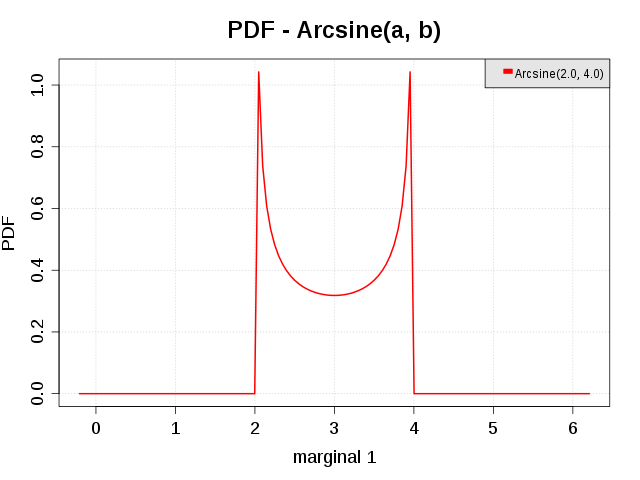
\includegraphics[width=7cm]{pdf_Arcsine.png}
      \caption{PDF of a Arcsine distribution.}
      \label{PDFArcsine}
    \end{center}
  \end{minipage}
  \hfill
  \begin{minipage}{10cm}
    \begin{center}
      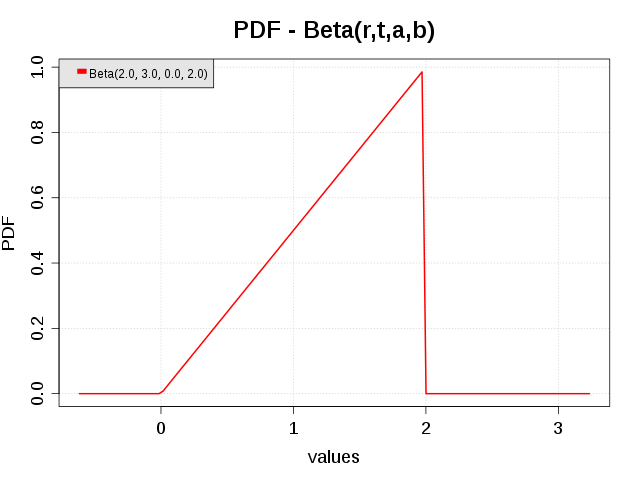
\includegraphics[width=7cm]{pdf_Beta_1.png}
      \caption{PDF of a Beta distribution.}
      \label{PDFBeta1}
    \end{center}
  \end{minipage}
\end{figure}

\begin{figure}[H]
  \begin{minipage}{10cm}
    \begin{center}
      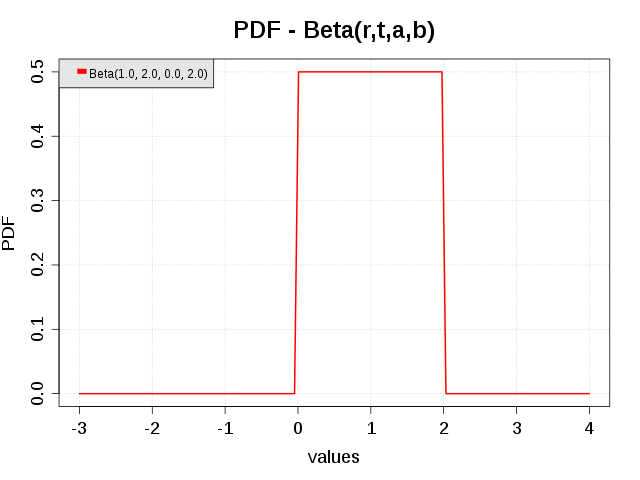
\includegraphics[width=7cm]{pdf_Beta_2.png}
      \caption{PDF of a Beta distribution.}
      \label{PDFBeta2}
    \end{center}
  \end{minipage}
  \hfill
  \begin{minipage}{10cm}
    \begin{center}
      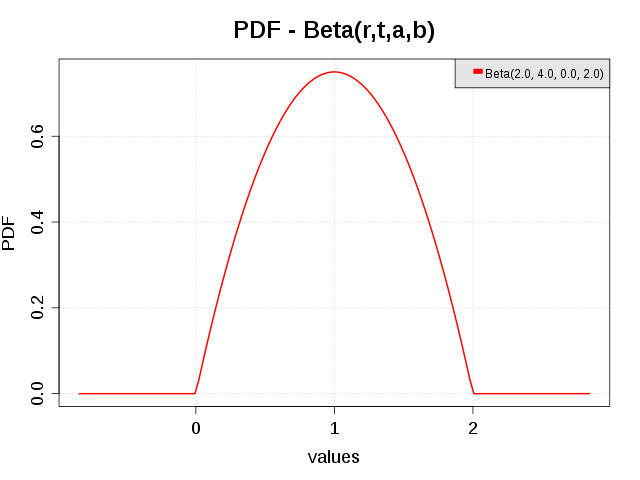
\includegraphics[width=7cm]{pdf_Beta_3.png}
      \caption{PDF of a Beta distribution.}
      \label{PDFBeta3}
    \end{center}
  \end{minipage}
\end{figure}

\begin{figure}[H]
  \begin{minipage}{10cm}
    \begin{center}
      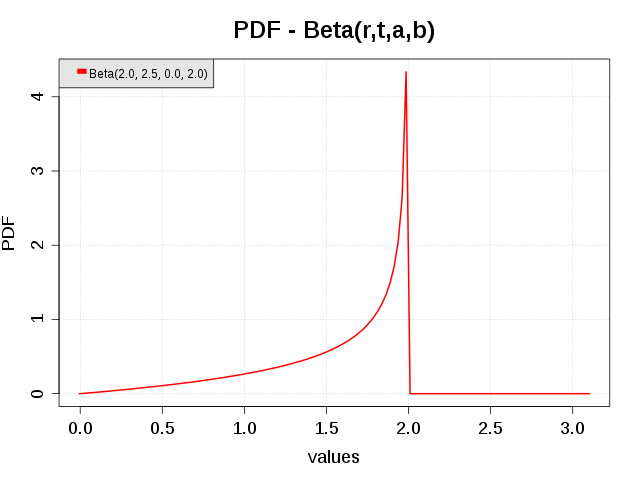
\includegraphics[width=7cm]{pdf_Beta_4.png}
      \caption{PDF of a Beta distribution.}
      \label{PDFBeta4}
    \end{center}
  \end{minipage}
  \hfill
  \begin{minipage}{10cm}
    \begin{center}
      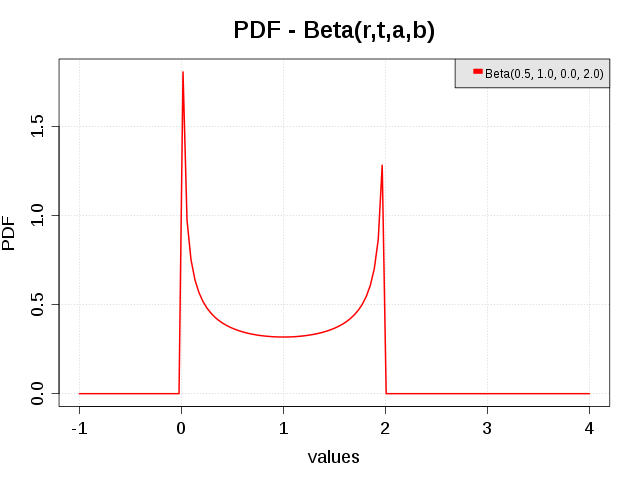
\includegraphics[width=7cm]{pdf_Beta_5.png}
      \caption{PDF of a Beta distribution.}
      \label{PDFBeta5}
    \end{center}
  \end{minipage}
\end{figure}


\begin{figure}[H]
  \begin{minipage}{10cm}
    \begin{center}
      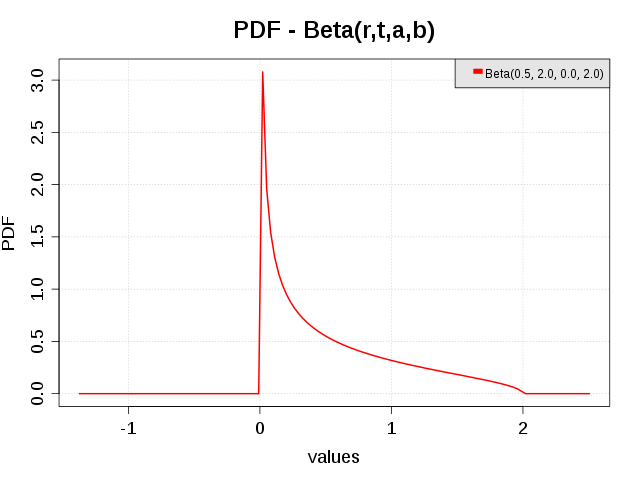
\includegraphics[width=7cm]{pdf_Beta_6.png}
      \caption{PDF of a Beta distribution.}
      \label{PDFBeta6}
    \end{center}
  \end{minipage}
  \hfill
  \begin{minipage}{10cm}
    \begin{center}
      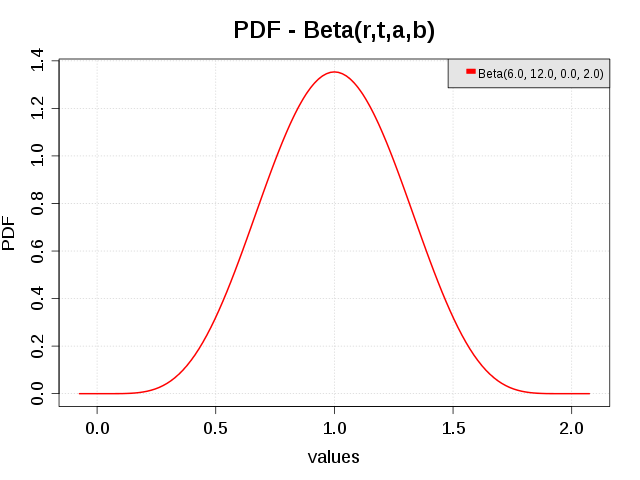
\includegraphics[width=7cm]{pdf_Beta_7.png}
      \caption{PDF of a Beta distribution.}
      \label{PDFBeta7}
    \end{center}
  \end{minipage}
\end{figure}


\begin{figure}[H]
  \begin{minipage}{10cm}
    \begin{center}
      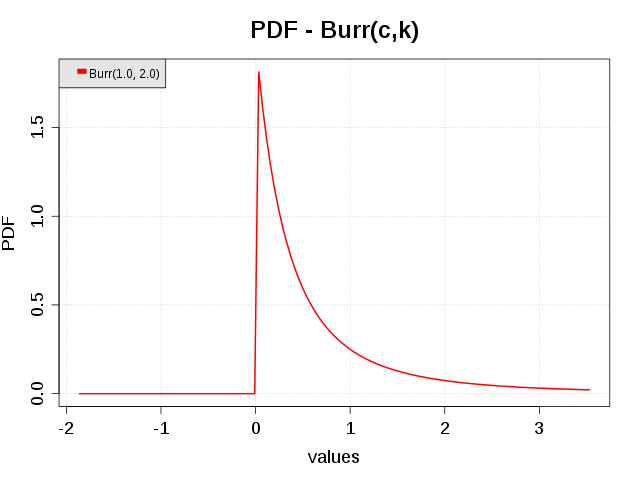
\includegraphics[width=7cm]{pdf_Burr_1.png}
      \caption{PDF of a Burr distribution.}
      \label{PDFBurr1}
    \end{center}
  \end{minipage}
  \hfill
  \begin{minipage}{10cm}
    \begin{center}
      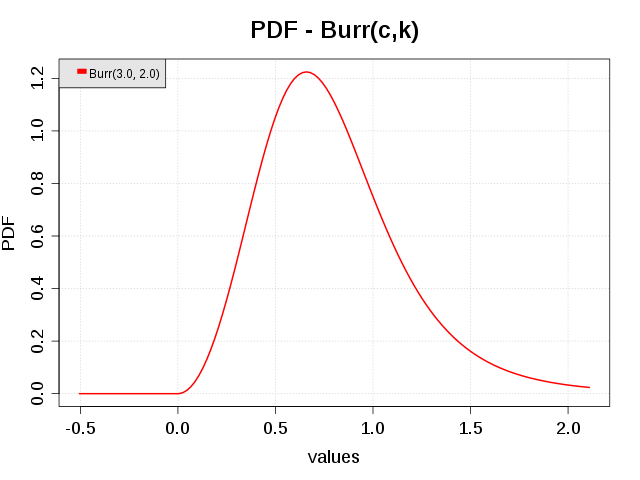
\includegraphics[width=7cm]{pdf_Burr_2.png}
      \caption{PDF of a Burr distribution.}
      \label{PDFBurr2}
    \end{center}
  \end{minipage}
\end{figure}


\begin{figure}[H]
  \begin{minipage}{10cm}
    \begin{center}
      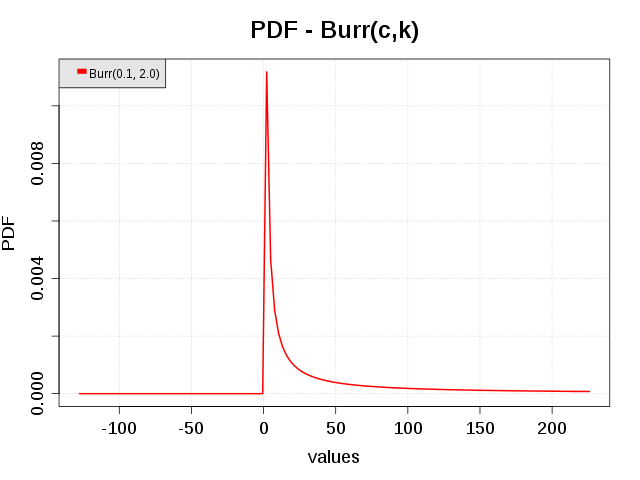
\includegraphics[width=7cm]{pdf_Burr_3.png}
      \caption{PDF of a Burr distribution.}
      \label{PDFBurr3}
    \end{center}
  \end{minipage}
  \hfill
  \begin{minipage}{10cm}
    \begin{center}
      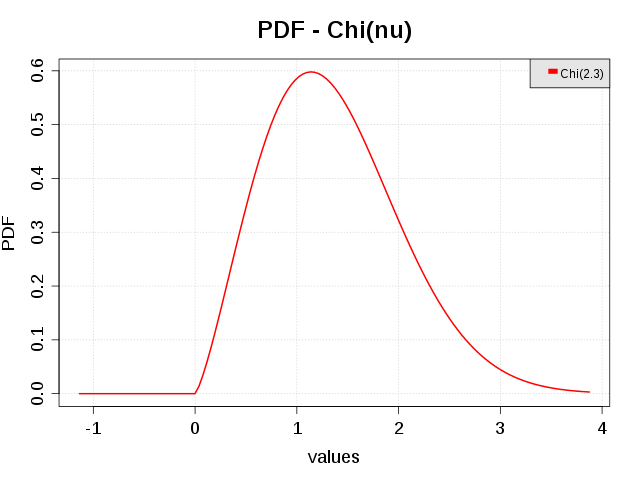
\includegraphics[width=7cm]{pdf_Chi_1.png}
      \caption{PDF of a Chi distribution.}
      \label{PDFChi1}
    \end{center}
  \end{minipage}
\end{figure}


\begin{figure}[H]
  \begin{minipage}{10cm}
    \begin{center}
      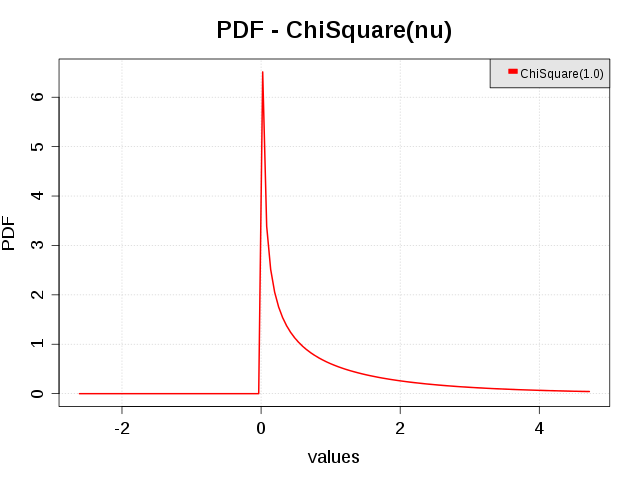
\includegraphics[width=7cm]{pdf_ChiSquare_1}
      \caption{PDF of a Chi Square distribution.}
      \label{PDFChiSquare1}
    \end{center}
  \end{minipage}
  \hfill
  \begin{minipage}{10cm}
    \begin{center}
      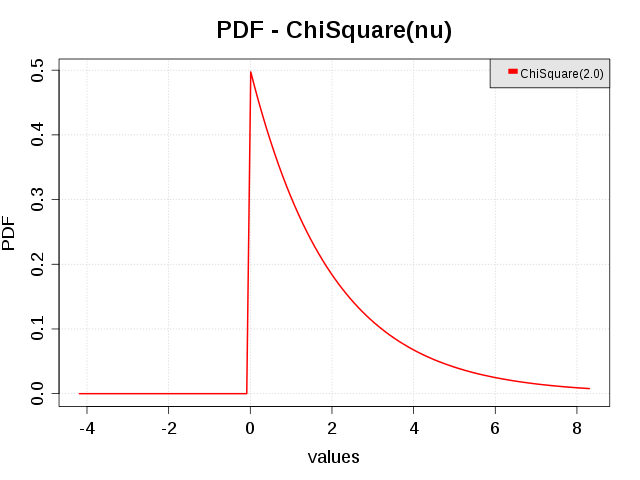
\includegraphics[width=7cm]{pdf_ChiSquare_2.png}
      \caption{PDF of a Chi Square distribution.}
      \label{PDFChiSquare2}
    \end{center}
  \end{minipage}
\end{figure}


\begin{figure}[H]
  \begin{minipage}{10cm}
    \begin{center}
      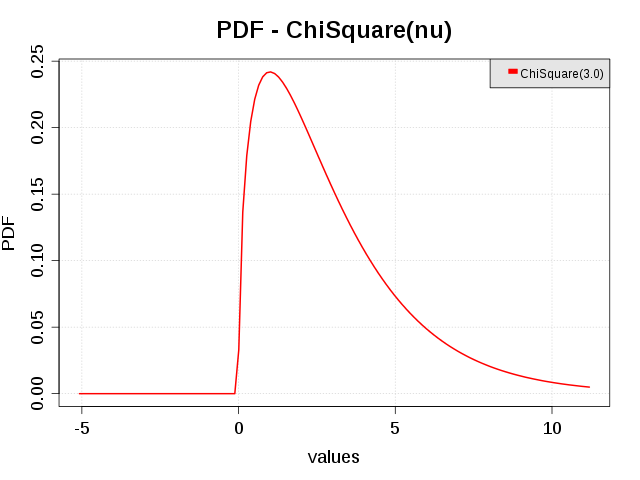
\includegraphics[width=7cm]{pdf_ChiSquare_3.png}
      \caption{PDF of a Chi Square distribution.}
      \label{PDFChiSquare3}
    \end{center}
  \end{minipage}
  \hfill
  \begin{minipage}{10cm}
    \begin{center}
      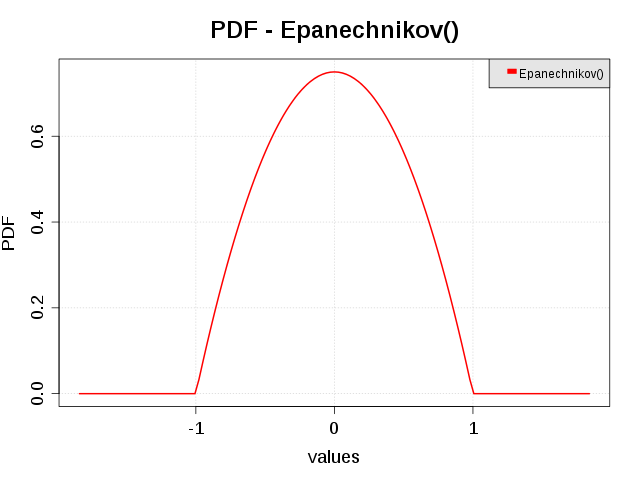
\includegraphics[width=7cm]{pdf_Epanechnikov.png}
      \caption{PDF of an Epanechnikov distribution.}
      \label{PDFEpanechnikov}
    \end{center}
  \end{minipage}
\end{figure}


\begin{figure}[H]
  \begin{minipage}{10cm}
    \begin{center}
      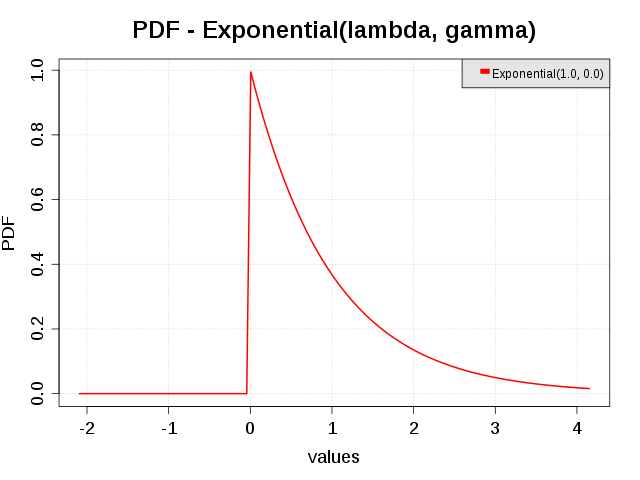
\includegraphics[width=7cm]{pdf_Exponential.png}
      \caption{PDF of a Exponential distribution.}
      \label{PDFExponential}
    \end{center}
  \end{minipage}
  \hfill
  \begin{minipage}{10cm}
    \begin{center}
      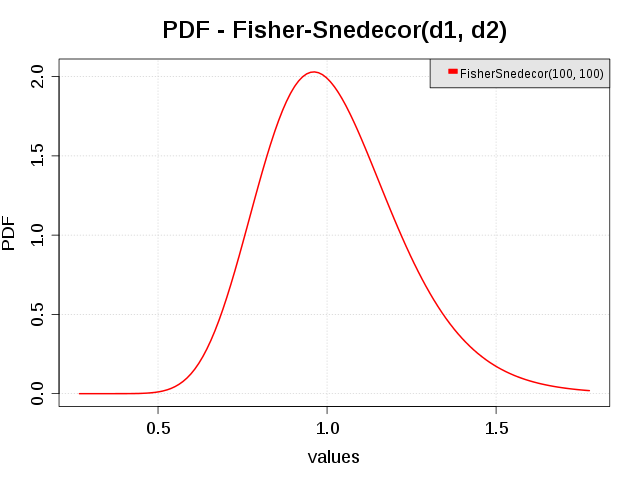
\includegraphics[width=7cm]{pdf_FisherSnedecor_1.png}
      \caption{PDF of a Fisher-Snedecor distribution.}
      \label{PDFFisherSnedecor1}
    \end{center}
  \end{minipage}
\end{figure}



\begin{figure}[H]
  \begin{minipage}{10cm}
    \begin{center}
      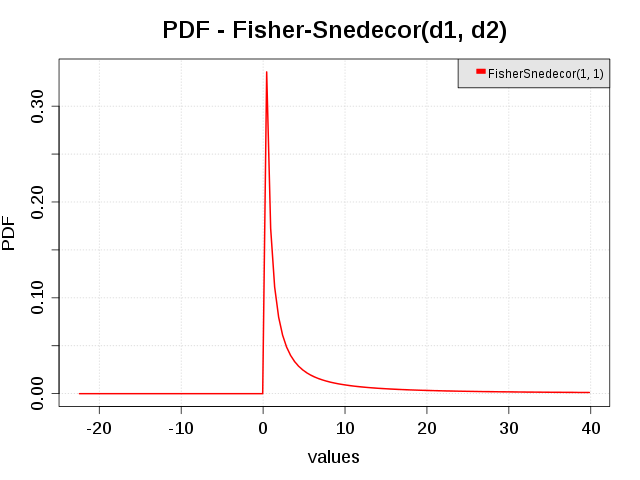
\includegraphics[width=7cm]{pdf_FisherSnedecor_2.png}
      \caption{PDF of a Fisher-Snedecor distribution.}
      \label{PDFFisherSnedecor2}
    \end{center}
  \end{minipage}
  \hfill
  \begin{minipage}{10cm}
    \begin{center}
      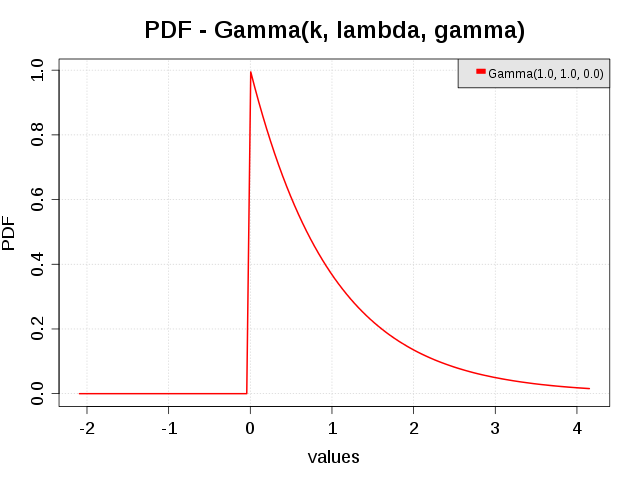
\includegraphics[width=7cm]{pdf_Gamma_1.png}
      \caption{PDF of a Gamma distribution.}
      \label{PDFGamma1}
    \end{center}
  \end{minipage}
\end{figure}

\begin{figure}[H]
  \begin{minipage}{10cm}
    \begin{center}
      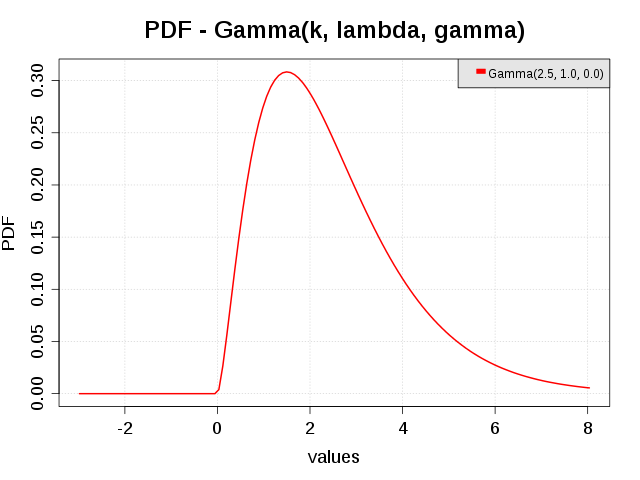
\includegraphics[width=7cm]{pdf_Gamma_2.png}
      \caption{PDF of a Gamma distribution.}
      \label{PDFGamma2}
    \end{center}
  \end{minipage}
  \hfill
  \begin{minipage}{10cm}
    \begin{center}
      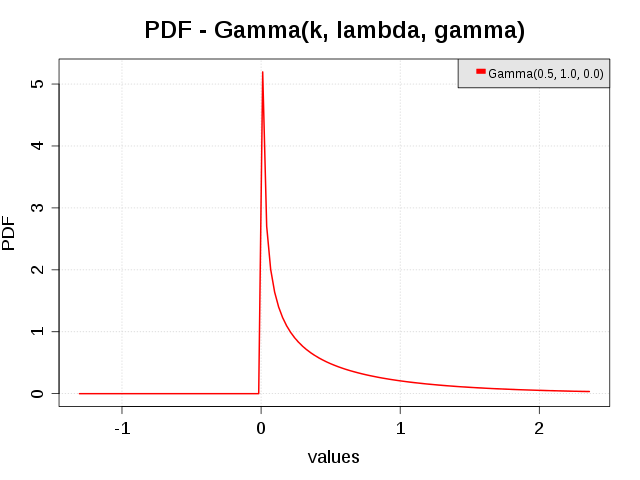
\includegraphics[width=7cm]{pdf_Gamma_3.png}
      \caption{PDF of a Gamma distribution.}
      \label{PDFGamma3}
    \end{center}
  \end{minipage}
\end{figure}




\begin{figure}[H]
  \begin{minipage}{10cm}
    \begin{center}
      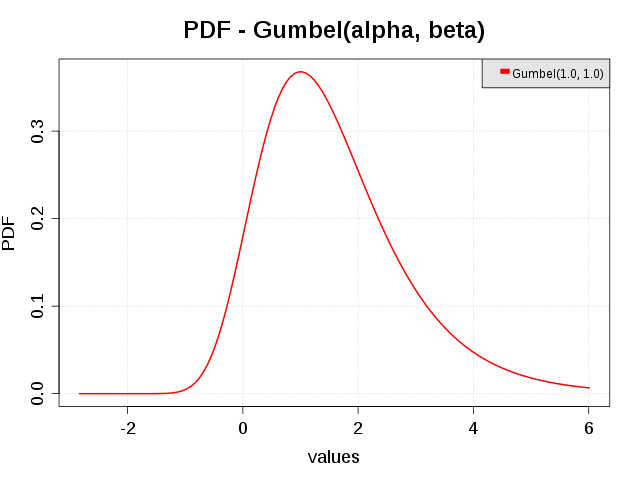
\includegraphics[width=7cm]{pdf_Gumbel.png}
      \caption{PDF of a Gumbel distribution.}
      \label{PDFGumbel}
    \end{center}
  \end{minipage}
  \hfill
  \begin{minipage}{10cm}
    \begin{center}
      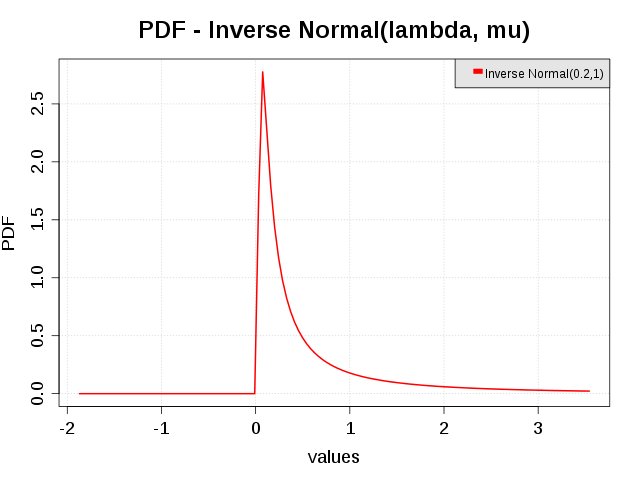
\includegraphics[width=7cm]{pdf_InverseNormal_1.png}
      \caption{PDF of a InverseNormal distribution.}
      \label{PDFInverseNormal1}
    \end{center}
  \end{minipage}
\end{figure}




\begin{figure}[H]
  \begin{minipage}{10cm}
    \begin{center}
      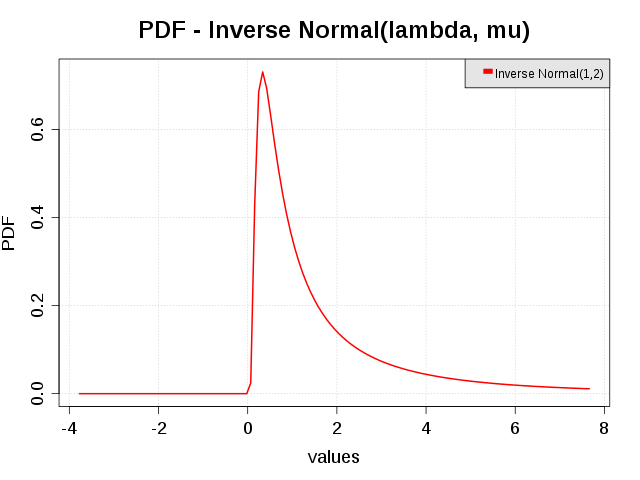
\includegraphics[width=7cm]{pdf_InverseNormal_2.png}
      \caption{PDF of a InverseNormal distribution.}
      \label{PDFInverseNormal2}
    \end{center}
  \end{minipage}
  \hfill
  \begin{minipage}{10cm}
    \begin{center}
      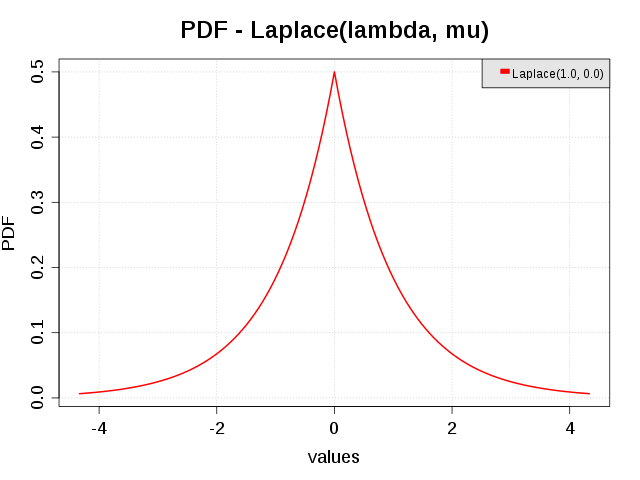
\includegraphics[width=7cm]{pdf_Laplace.png}
      \caption{PDF of a Laplace distribution.}
      \label{PDFLaplace}
    \end{center}
  \end{minipage}
\end{figure}




\begin{figure}[H]
  \begin{minipage}{10cm}
    \begin{center}
      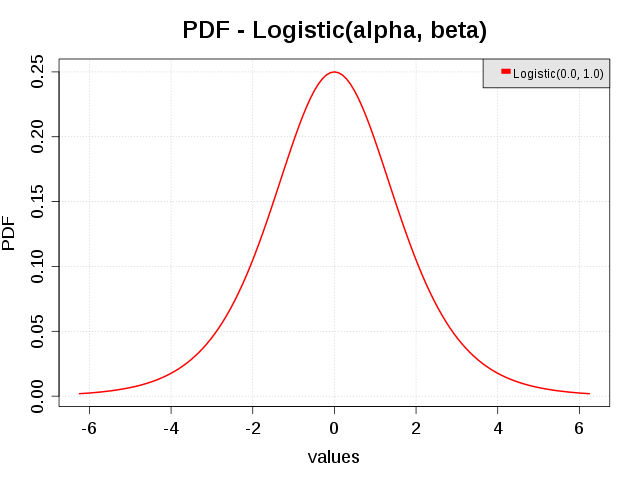
\includegraphics[width=7cm]{pdf_Logistic.png}
      \caption{PDF of a Logistic distribution.}
      \label{PDFLogistic}
    \end{center}
  \end{minipage}
  \hfill
  \begin{minipage}{10cm}
    \begin{center}
      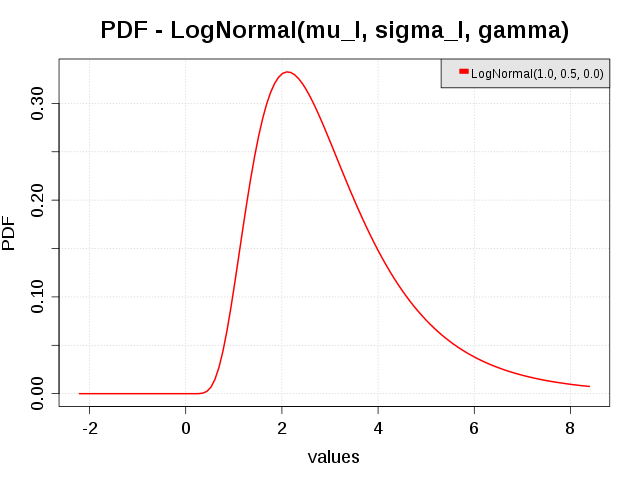
\includegraphics[width=7cm]{pdf_LogNormal.png}
      \caption{PDF of a  LogNormal distribution.}
      \label{PDFLogNormal}
    \end{center}
  \end{minipage}
\end{figure}






\begin{figure}[H]
  \begin{minipage}{10cm}
    \begin{center}
      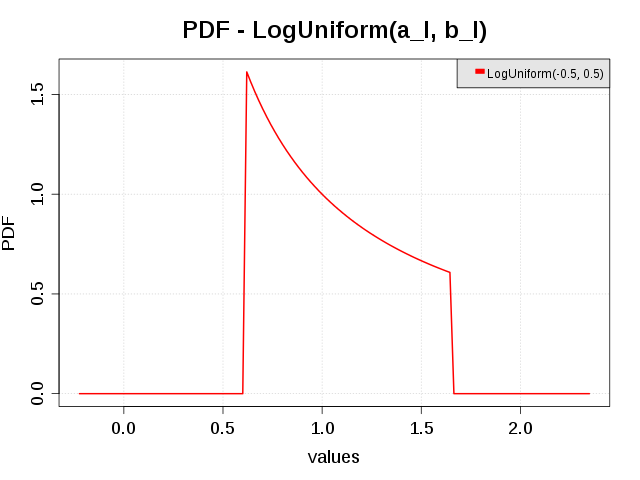
\includegraphics[width=7cm]{pdf_LogUniform.png}
      \caption{PDF of a  LogUniform distribution.}
      \label{PDFLogUniform}
    \end{center}
  \end{minipage}
  \hfill
  \begin{minipage}{10cm}
    \begin{center}
      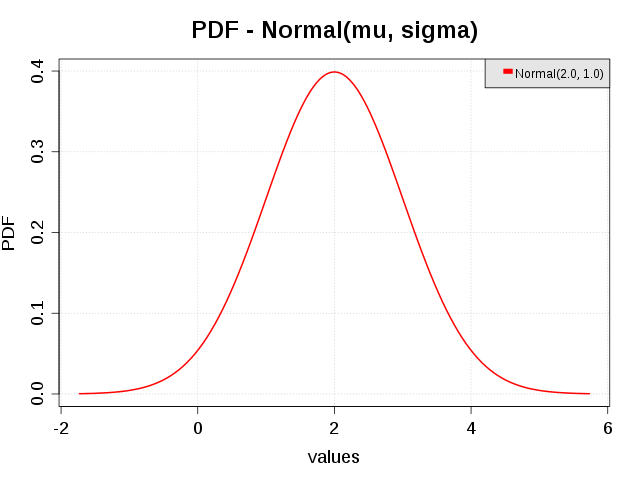
\includegraphics[width=7cm]{pdf_Normal.png}
      \caption{PDF of a Normal distribution.}
      \label{PDFNormal}
    \end{center}
  \end{minipage}
\end{figure}



\begin{figure}[H]
  \begin{minipage}{10cm}
    \begin{center}
      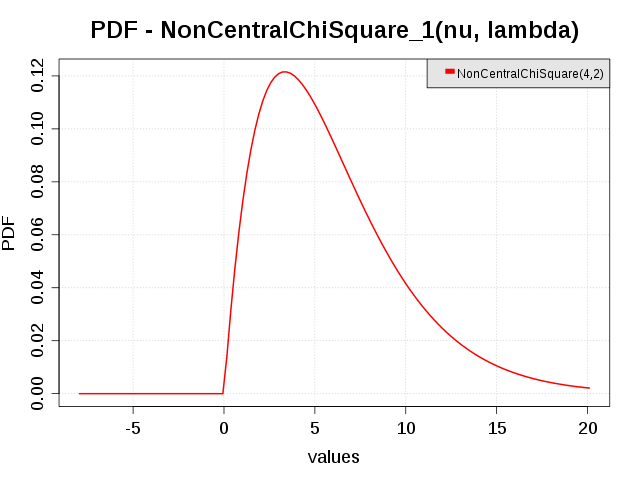
\includegraphics[width=7cm]{pdf_NonCentralChiSquare_1.png}
      \caption{PDF of a Non Central Chi Square distribution.}
      \label{PDFNonCentralChiSquare1}
    \end{center}
  \end{minipage}
  \hfill
  \begin{minipage}{10cm}
    \begin{center}
      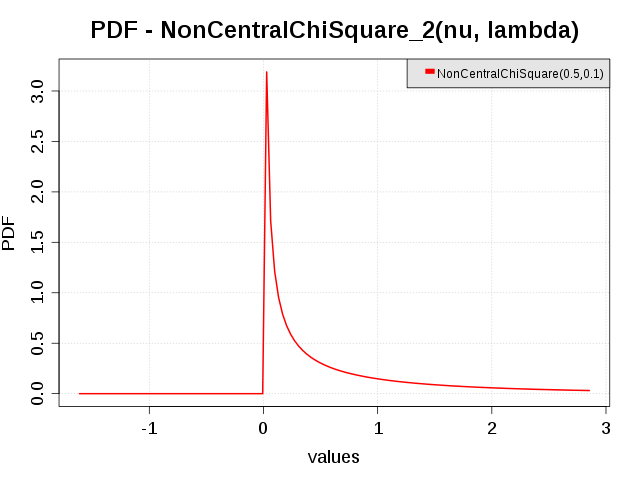
\includegraphics[width=7cm]{pdf_NonCentralChiSquare_2.png}
      \caption{PDF of a Non Central Chi Square distribution.}
      \label{PDFNonCentralChiSquare2}
    \end{center}
  \end{minipage}
\end{figure}


\begin{figure}[H]
  \begin{minipage}{10cm}
    \begin{center}
      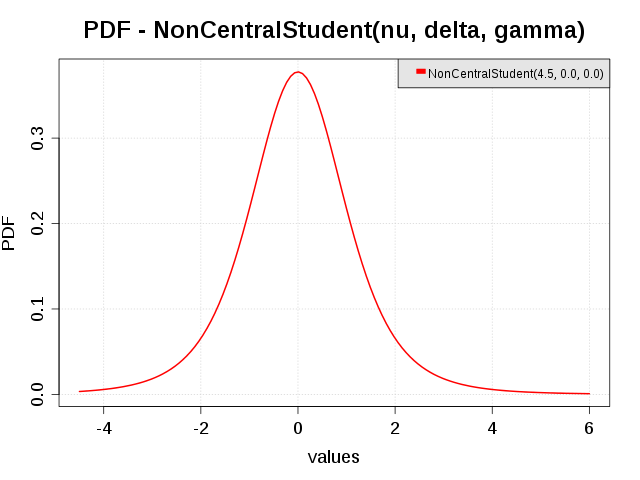
\includegraphics[width=7cm]{pdf_NonCentralStudent.png}
      \caption{PDF of a Non Central Student distribution.}
      \label{PDFNonCentralStudent}
    \end{center}
  \end{minipage}
  \hfill
  \begin{minipage}{10cm}
    \begin{center}
      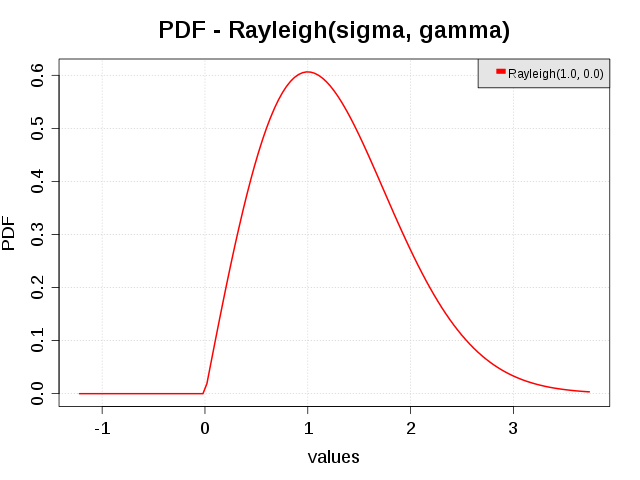
\includegraphics[width=7cm]{pdf_Rayleigh.png}
      \caption{PDF of a Rayleigh distribution.}
      \label{PDFRayleigh}
    \end{center}
  \end{minipage}
\end{figure}


\begin{figure}[H]
  \begin{minipage}{10cm}
    \begin{center}
      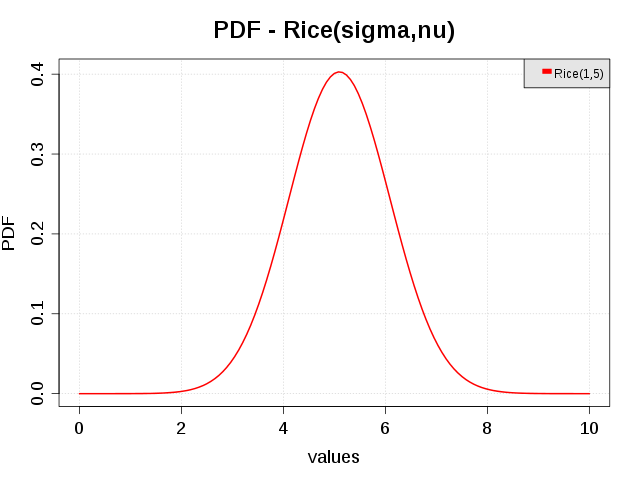
\includegraphics[width=7cm]{pdf_Rice_1.png}
      \caption{PDF of a Rice distribution.}
      \label{PDFRice1}
    \end{center}
  \end{minipage}
  \hfill
  \begin{minipage}{10cm}
    \begin{center}
      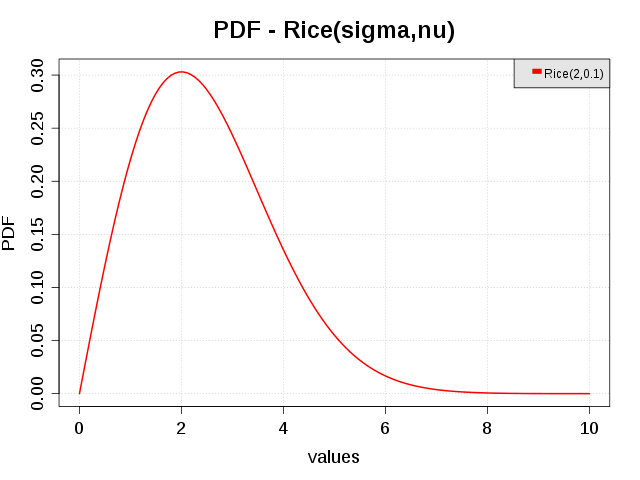
\includegraphics[width=7cm]{pdf_Rice_2.png}
      \caption{PDF of a Rice distribution.}
      \label{PDFRice2}
    \end{center}
  \end{minipage}
\end{figure}


\begin{figure}[H]
  \begin{minipage}{10cm}
    \begin{center}
      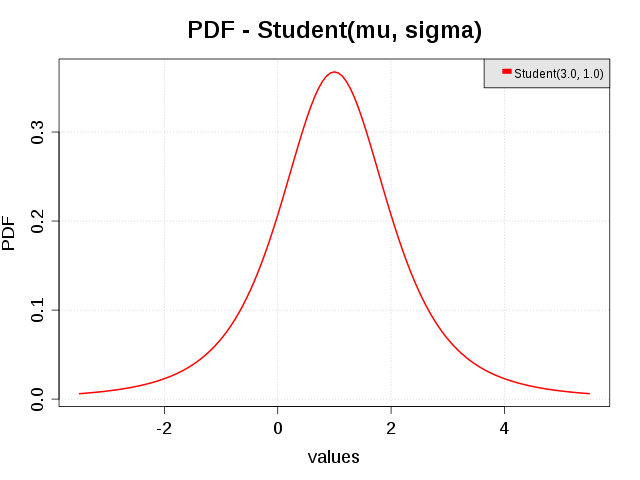
\includegraphics[width=7cm]{pdf_Student.png}
      \caption{PDF of a Student distribution.}
      \label{PDFStudent}
    \end{center}
  \end{minipage}
  \hfill
  \begin{minipage}{10cm}
    \begin{center}
      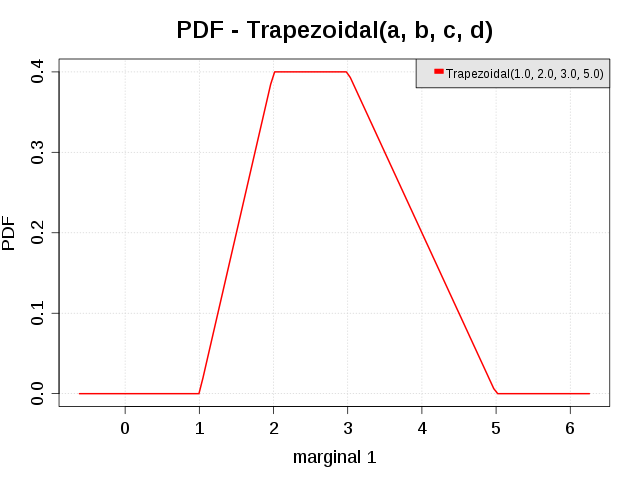
\includegraphics[width=7cm]{pdf_Trapezoidal.png}
      \caption{PDF of a Trapezoidal distribution.}
      \label{PDFTrapezoidal}
    \end{center}
  \end{minipage}
\end{figure}

\begin{figure}[H]
  \begin{minipage}{10cm}
    \begin{center}
      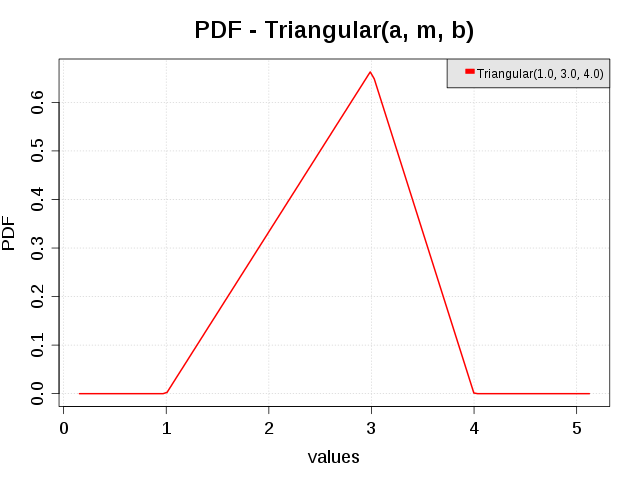
\includegraphics[width=7cm]{pdf_Triangular.png}
      \caption{PDF of a  Triangular distribution.}
      \label{PDFTriangular}
    \end{center}
  \end{minipage}
  \hfill
  \begin{minipage}{10cm}
    \begin{center}
      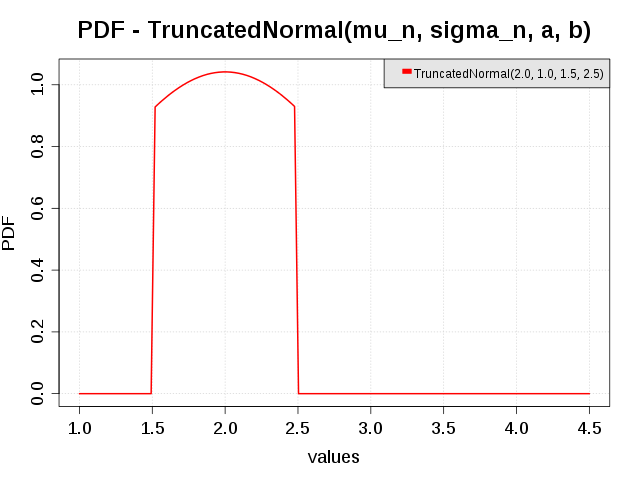
\includegraphics[width=7cm]{pdf_TruncatedNormal_1.png}
      \caption{PDF of a  Truncated Normal distribution.}
      \label{PDFTruncatedNormal1}
    \end{center}
  \end{minipage}
\end{figure}

\begin{figure}[H]
  \begin{minipage}{10cm}
    \begin{center}
      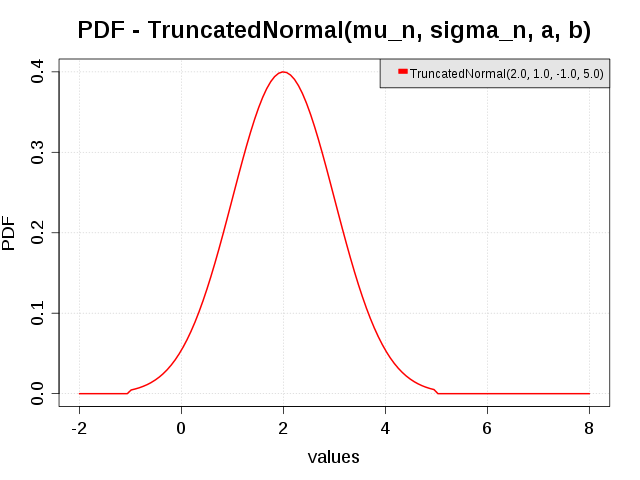
\includegraphics[width=7cm]{pdf_TruncatedNormal_2.png}
      \caption{PDF of a  Truncated Normal distribution.}
      \label{PDFTruncatedNormal2}
    \end{center}
  \end{minipage}
  \hfill
  \begin{minipage}{10cm}
    \begin{center}
      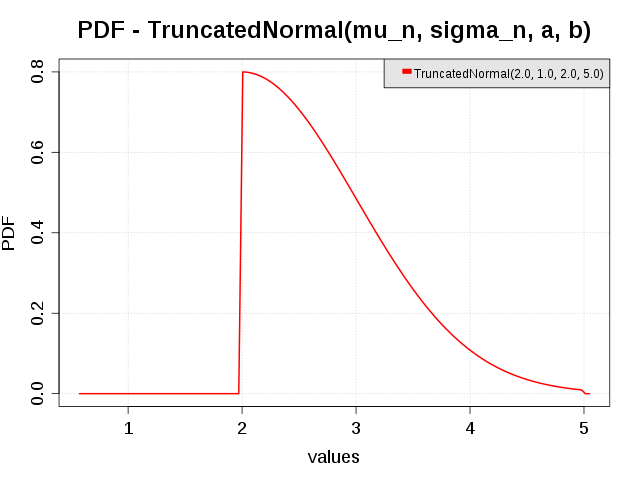
\includegraphics[width=7cm]{pdf_TruncatedNormal_3.png}
      \caption{PDF of a  Truncated Normal distribution.}
      \label{PDFTruncatedNormal3}
    \end{center}
  \end{minipage}
\end{figure}

\begin{figure}[H]
  \begin{minipage}{10cm}
    \begin{center}
      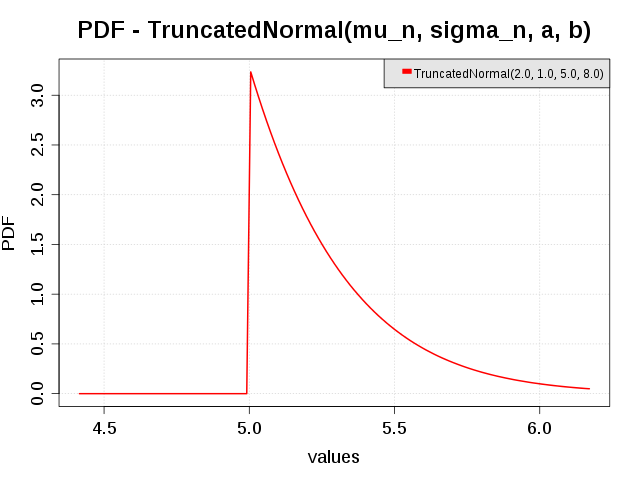
\includegraphics[width=7cm]{pdf_TruncatedNormal_4.png}
      \caption{PDF of a  TruncatedNormaldistribution.}
      \label{PDFTruncatedNormal4}
    \end{center}
  \end{minipage}
  \hfill
  \begin{minipage}{10cm}
    \begin{center}
      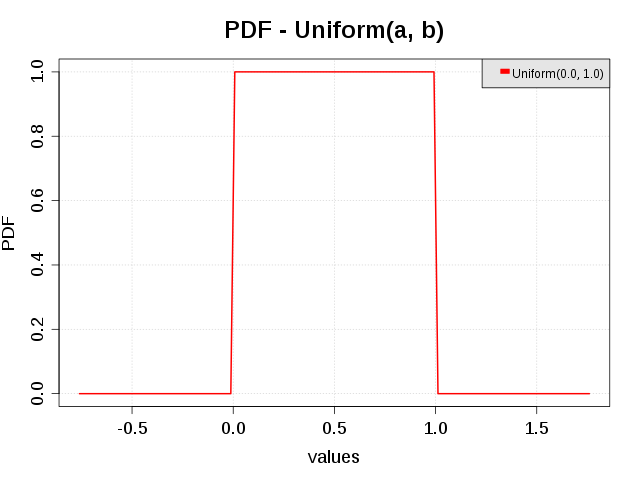
\includegraphics[width=7cm]{pdf_Uniform.png}
      \caption{PDF of a  Uniform distribution.}
      \label{PDFUniform}
    \end{center}
  \end{minipage}
\end{figure}




\begin{figure}[H]
  \begin{minipage}{10cm}
    \begin{center}
      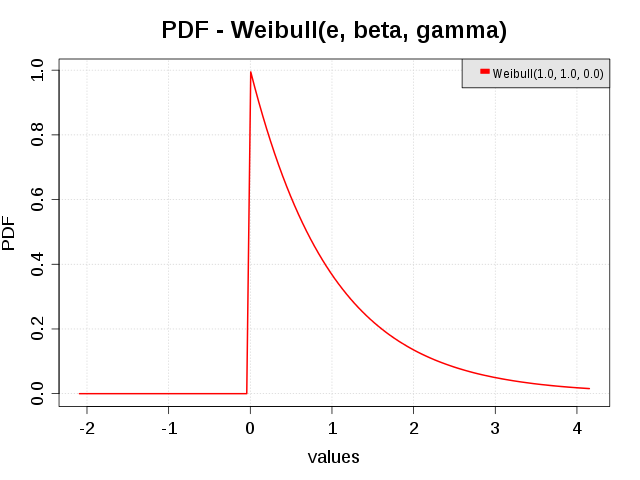
\includegraphics[width=7cm]{pdf_Weibull_1.png}
      \caption{PDF of a  Weibull distribution.}
      \label{PDFWeibull1}
    \end{center}
  \end{minipage}
  \hfill
  \begin{minipage}{10cm}
    \begin{center}
      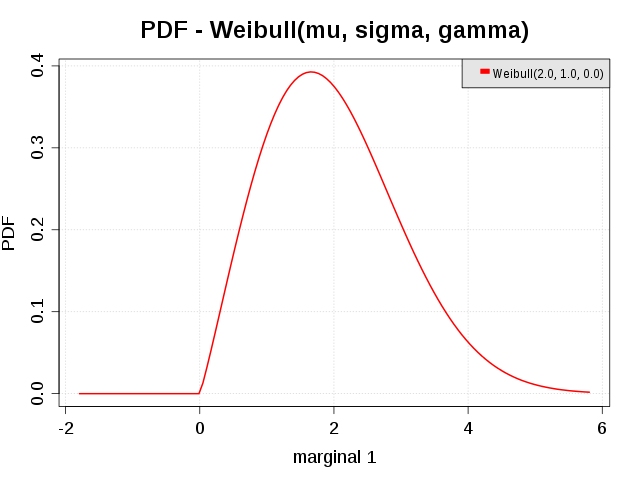
\includegraphics[width=7cm]{pdf_Weibull_2.png}
      \caption{PDF of a Weibull distribution.}
      \label{PDFWeibull2}
    \end{center}
  \end{minipage}
\end{figure}





The Histogram distribution explicited in the Use Case is drawn in Figures \ref{PDFHistogram} and \ref{CDFHistogram}.

\begin{figure}[H]
  \begin{minipage}{10cm}
    \begin{center}
      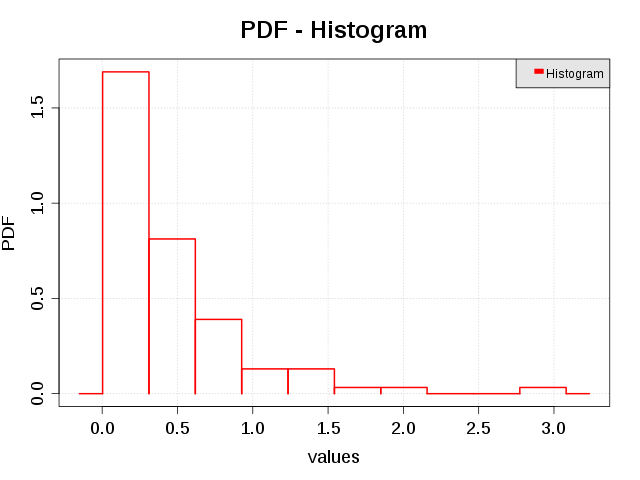
\includegraphics[width=7cm]{pdf_Histogram.png}
      \caption{PDF of an Histogram distribution.}
      \label{PDFHistogram}
    \end{center}
  \end{minipage}
  \hfill
  \begin{minipage}{10cm}
    \begin{center}
      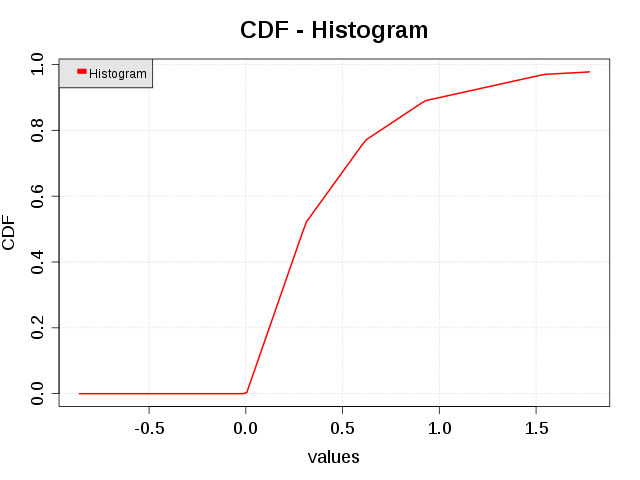
\includegraphics[width=7cm]{cdf_Histogram.png}
      \caption{CDF of an Histogram distribution.}
      \label{CDFHistogram}
    \end{center}
  \end{minipage}
\end{figure}




The discrete distributions explicited in the Use Case  have the following distribution graphs, drawn in Figures \ref{PDFBernoulli} to Figure \ref{CDFUserDefined}.



\begin{figure}[H]
  \begin{minipage}{10cm}
    \begin{center}
      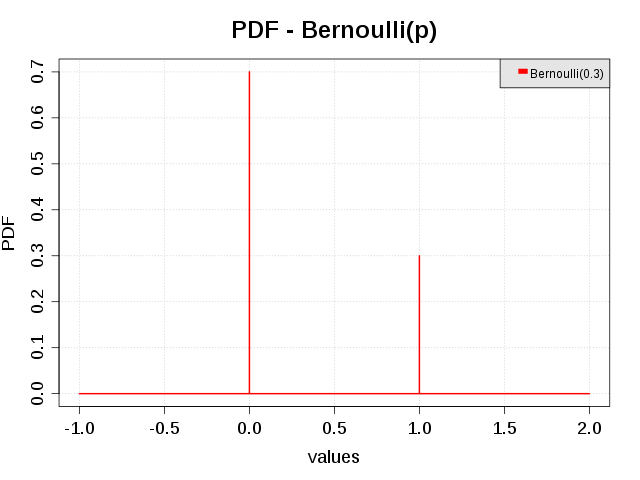
\includegraphics[width=7cm]{pdf_Bernoulli.png}
      \caption{Distribution of a Bernoulli distribution.}
      \label{PDFBernoulli}
    \end{center}
  \end{minipage}
  \hfill
  \begin{minipage}{10cm}
    \begin{center}
      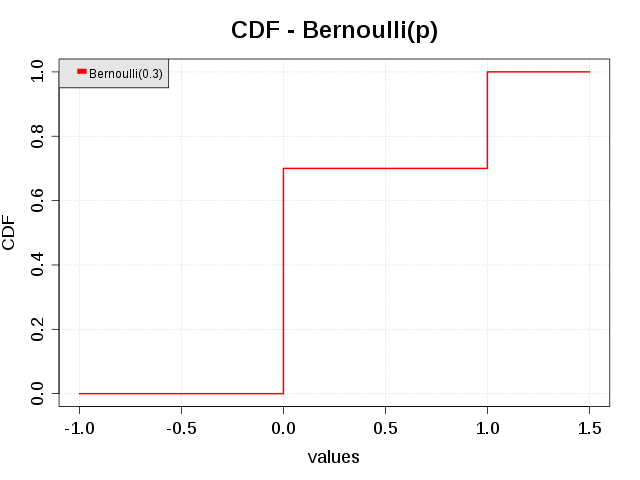
\includegraphics[width=7cm]{cdf_Bernoulli.png}
      \caption{CDF of a Bernoulli distribution.}
      \label{CDFBernoulli}
    \end{center}
  \end{minipage}
\end{figure}





\begin{figure}[H]
  \begin{minipage}{10cm}
    \begin{center}
      \includegraphics[width=7cm]{pdf_Binomial.png}
      \caption{Distribution of a Binomial distribution.}
      \label{PDFBinomial}
    \end{center}
  \end{minipage}
  \hfill
  \begin{minipage}{10cm}
    \begin{center}
      \includegraphics[width=7cm]{cdf_Binomial.png}
      \caption{CDF of a Binomial distribution.}
      \label{CDFBinomial}
    \end{center}
  \end{minipage}
\end{figure}



\begin{figure}[H]
  \begin{minipage}{10cm}
    \begin{center}
      \includegraphics[width=7cm]{pdf_Geometric.png}
      \caption{Distribution of a Geometric distribution.}
      \label{PDFGeometric}
    \end{center}
  \end{minipage}
  \hfill
  \begin{minipage}{10cm}
    \begin{center}
      \includegraphics[width=7cm]{cdf_Geometric.png}
      \caption{CDF of a Geometric distribution.}
      \label{CDFGeometric}
    \end{center}
  \end{minipage}
\end{figure}



\begin{figure}[H]
  \begin{minipage}{10cm}
    \begin{center}
      \includegraphics[width=7cm]{pdf_Poisson.png}
      \caption{Distribution of a Poisson distribution.}
      \label{PDFPoisson}
    \end{center}
  \end{minipage}
  \hfill
  \begin{minipage}{10cm}
    \begin{center}
      \includegraphics[width=7cm]{cdf_Poisson.png}
      \caption{CDF of a Poisson distribution.}
      \label{CDFPoisson}
    \end{center}
  \end{minipage}
\end{figure}



\begin{figure}[H]
  \begin{minipage}{10cm}
    \begin{center}
      \includegraphics[width=7cm]{pdf_UserDefined.png}
      \caption{Distribution of a  UserDefined distribution.}
      \label{PDFUserDefined}
    \end{center}
  \end{minipage}
  \hfill
  \begin{minipage}{10cm}
    \begin{center}
      \includegraphics[width=7cm]{cdf_UserDefined.png}
      \caption{CDF of a UserDefined distribution.}
      \label{CDFUserDefined}
    \end{center}
  \end{minipage}
\end{figure}



\begin{figure}[H]
  \begin{minipage}{10cm}
    \begin{center}
      \includegraphics[width=7cm]{pdf_ZipfMandelbrot_1.png}
      \caption{Distribution of a  Zipf-Mandelbrot distribution.}
      \label{PDFZipfMandelbrot}
    \end{center}
  \end{minipage}
  \hfill
  \begin{minipage}{10cm}
    \begin{center}
      \includegraphics[width=7cm]{cdf_ZipfMandelbrot_1.png}
      \caption{CDF of a Zipf-Mandelbrot  distribution.}
      \label{CDFZipfMandelbrot}
    \end{center}
  \end{minipage}
\end{figure}

